% UTF-8 encoding
% Compile with latex+dvipdfmx, pdflatex, xelatex or lualatex

\documentclass[hyperref, UTF8]{ctexart}
\usepackage{graphicx}
\usepackage{amssymb}
\usepackage{amsmath}
\usepackage{subfigure}
\usepackage{geometry}
\usepackage{caption}
\newcommand{\volt}{{\rm V}}
\newcommand{\source}{{\rm S}}
\newcommand{\ampere}{{\rm A}}
\newcommand{\ohm}{\Omega}
\newcommand{\kiloohm}{{\rm k}\Omega}
\newcommand{\watt}{{\rm W}}
\newcommand{\kilowatt}{{\rm kW}}

\title{电子学基础——第三次作业}
\author{LXQ}
\date{2019.09.30}

\geometry{left=2.0cm, right=2.0cm, top=2.5cm, bottom=2.5cm}
\linespread{1}

\begin{document}

\maketitle

\paragraph{4-15}\label{4-15}
利用电源变换,求题图4-15所示电路的戴维南等效电路。

\begin{figure}[!htb]
\centering
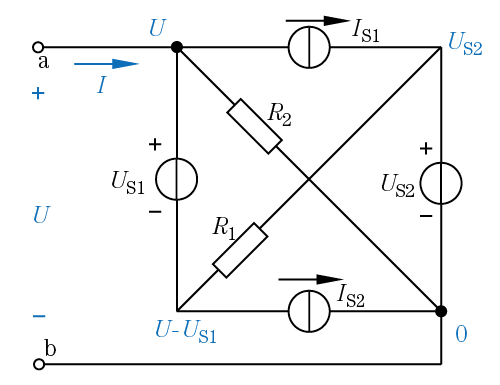
\includegraphics[width=0.333\textwidth]{p4-15.png}
\caption*{题图 4-15}
\end{figure}

\paragraph{解}如图所示,设干路电流为$I$,端口电压为$U$。记$\rm b$端为$0$电势点,其余各点电势如图所示。则可列写方程:
\begin{gather*}
U = R_2[I - I_{\source 1} - (I_{\source 2} + \frac{U-U_{\source 1}-U_{\source 2}}{R_1})] \\
\therefore U = \frac{R_2(U_{\source 1}+U_{\source 2}) - R_1R_2(I_{\source 1}+I_{\source 2})}{R_1+R_2} + \frac{R_1R_2}{R_1+R_2}I
\end{gather*}

则戴维南等效电路如图4-15所示,其中
\begin{gather*}
U_{\rm eq}=\frac{R_2(U_{\source 1}+U_{\source 2}) - R_1R_2(I_{\source 1}+I_{\source 2})}{R_1+R_2} \\
R_{\rm eq}=\frac{R_1R_2}{R_1+R_2}
\end{gather*}

\begin{figure}[!htb]
\centering
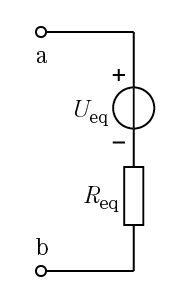
\includegraphics[width=0.120\textwidth]{p4-15-sol.png}
\caption*{图 4-15}
\end{figure}

\paragraph{4-25}\label{4-25}
试求出题图4-25所示的二端网络的戴维南等效电路和诺顿等效电路。

\begin{figure}[!htb]
\centering
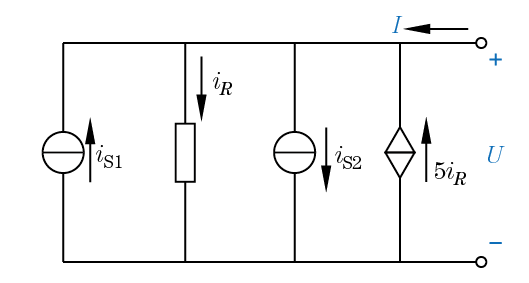
\includegraphics[width=0.353\textwidth]{p4-25.png}
\caption*{题图 4-25}
\end{figure}

\paragraph{解}如图所示,设干路电流为$I$,端口电压为$U$。则可列写方程:
\begin{gather*}
i_R=I+i_{\source 1}+5i_R-i_{\source 2} \\
\therefore U = Ri_R = R \cdot \frac{i_{\source 1}-i_{\source 2}-I}{4} \\
\therefore U = \frac{R(i_{\source 2}-i_{\source 1})}{4} - \frac{R}{4}I \\
I = -\frac{4U}{R} - i_{\source 1} + i_{\source 2}
\end{gather*}

则戴维南电路如图4-25 (a) 所示,其中
$$
U_{\rm eq}=\frac{R(i_{\source 2}-i_{\source 1})}{4}, 
R_{\rm eq}= - \frac{R}{4} 
$$

诺顿电路如图4-25 (b) 所示,其中
$$
I_{\rm eq}= - i_{\source 1} + i_{\source 2},
S_{\rm eq}= -\frac{4}{R}
$$

\begin{figure}[!htb]
\centering
\begin{minipage}[t]{0.179\textwidth}
\centering
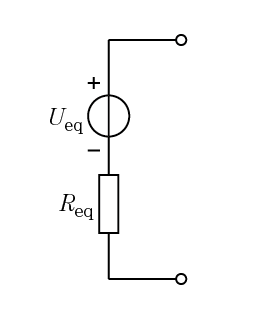
\includegraphics[width=1\textwidth]{p4-25-sol1.png}
\caption*{(a)}
\end{minipage}
\begin{minipage}[t]{0.210\textwidth}
\centering
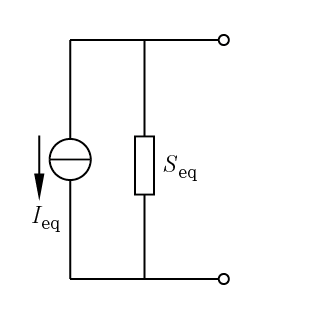
\includegraphics[width=1\textwidth]{p4-25-sol2.png}
\caption*{(b)}
\end{minipage}
\caption*{图 4-25}
\end{figure}

\paragraph{4-45}\label{4-45}
题图4-45所示电路中,$\rm N$为无源线性电阻网络。当$R_2=2\ohm$, $U_\source=6\volt$时,测得$I_1=2\ampere$, $U_2=2\volt$。如果当$R_2=4\ohm$, $U_s=10\volt$时,又测得$I_1=3\ampere$,求此时的电压$U_2$。

\begin{figure}[!htb]
\centering
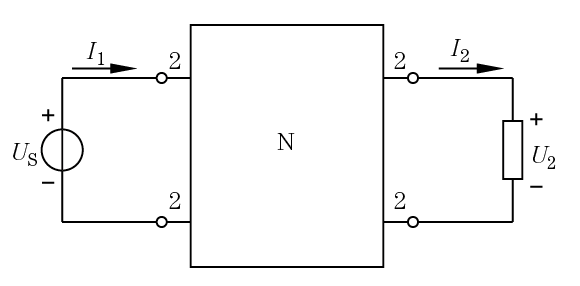
\includegraphics[width=0.387\textwidth]{p4-45.png}
\caption*{题图 4-45}
\end{figure}

\paragraph{解}
设$1$号端口电压与电流分别为$u_1=U_\source, i_1=-I_1$(取关联参考方向,下同),$2$号端口电压与电流分别为$u_2=U_2, i_2=I_2$。$N$中各支路电压、电流、电阻为$u_k, i_k, R_k$。为易于区分,第二次测量的各物理量用hat符号标记。\\

则由特勒根定理可知
\begin{gather*}
\left\{\begin{aligned}
\hat{u_1}i_1 + \sum_{k}\hat{u_k}i_k + \hat{u_2}i_2 &= 0 \\
u_1\hat{i_1} + \sum_{k}u_k\hat{i_k} + u_2\hat{i_2} &= 0
\end{aligned}\right.
\end{gather*}

由于$\sum_{k}\hat{u_k}i_k = \sum_{k}R_k\hat{i_k}i_k = \sum_{k}u_k\hat{i_k}$,则上述两式相减并带入数值可得
\begin{gather*}
10\times (-2) + \hat{u_2} = 6 \times (-3) + 2 \times \frac{\hat{u_2}}{4} \\
\therefore \hat{u_2}=4\volt
\end{gather*}

\end{document}